\subsection{CSS} % (fold)
\label{sub:css}

In the early years of the \ida{WWW}, as it was starting to hit the mainstream, web developers were asked to build visually attractive web pages.
\ida{HTML} was not prepared for this and the only way to do it was using a lot of tables and cropped images.
Inevitably, this always ends in a tag soup impossible to understand and even more difficult to maintain.

The \ida{W3C}, with \emph{Robert Cailliau} (\ida{WWW} co-founder) at its head, wanted a solution to separate the structure from the presentation.
That way the \ida{HTML} file would gather only the content and external style sheets would specify how to show that content (layout, colors, fonts, etc).

This separation is aimed at improving the accessibility of the page independently of how it is consumed (on screen, in print, by voice, etc).
Incidentally it provides more flexibility and control, avoiding repetition by sharing the same stylesheet between pages.
In most browsers, there are also options to override certain aspects of a page style, e.g. this is very useful for a visually impaired person.

\begin{wrapfigure}{r}{0.5\textwidth}
  \centering
    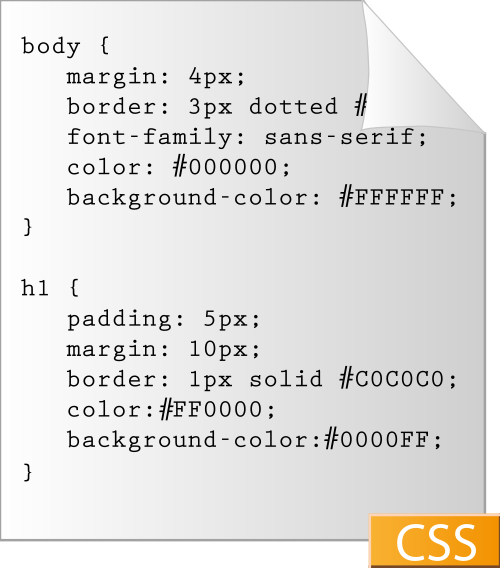
\includegraphics[width=0.48\textwidth]{css-source}
  \caption{Example \idx{CSS} source}
  \label{fig:css-source}
\end{wrapfigure}

After several proposals in this direction, \emph{Håkon Wium Lie} and \emph{Bert Bos} started working in the specification of \ida{CSS}, releasing the first version in 1996.
The second recommendation \ida{CSS} 2 was released less than two years later in 1998, and more than thirteen years later its successors (\ida{CSS} 2.1  \cite{CSS2} and \ida{CSS} 3) are yet to reach the \emph{Recommendation} status \cite{CSS}.
Almost full support for \ida{CSS} 2.1 is provided in every major browser and partial support for \ida{CSS} 3 is provided in modern browsers with uneven results.

A \ida{CSS} file defines a set of rules with properties to be applied to the elements of the page.
Each rule can affect several elements, and each element can be affected by several rules at the same time, so a priority system is needed to predictably decide with rule shall prevail in this \emph{cascade}.

Every rule consists of one or more \emph{selectors} and one or more properties stated inside the declaration block.
A selector is a pattern matching elements in the \ida{HTML} source.
Table~\vref{tab:cssselectors} contains all the available selectors in \ida{CSS} 2.1\footnote{The information depicted in Table~\vref{tab:cssselectors} has been extracted from the official specification documentation, specifically from here: \url{http://www.w3.org/TR/CSS2/selector.html}}.

Those selectors can be mixed and put together composing a more complex selector targeting specific elements.
When several selectors share the same declarations, they may be grouped into a comma-separated list to avoid repetition.
When there is a collision between two rules, the browser follows this simplified selector precedence: the selector with more ID attributes, the selector with more classes/attributes/pseudo-classes, the selector with more elements/pseudo-elements.
If two rules tie, the last declared rule is the winner.

\begin{generictable}[\idx{CSS} 2.1 selectors]{3}
  {|p{0.17\textwidth}|p{0.21\textwidth}|p{0.5\textwidth}|}
  {\generictitlethree{Pattern}{Type}{Meaning}}
  \label{tab:cssselectors}%
  \footnotesize{\verb|*|}
  & Universal\newline selector
  & Matches any element. \\ \hline
  \footnotesize{\verb|E|}
  & Type selector
  & Matches any E element (i.e., an element of type E). \\ \hline
  \footnotesize{\verb|E F|}
  & Descendant\newline selector
  & Matches any F element that is a descendant of an E element. \\ \hline
  \footnotesize{\verb|E > F|}
  & Child selector
  & Matches any F element that is a child of an element E. \\ \hline
  \footnotesize{\verb|E + F|}
  & Adjacent\newline selector
  & Matches any F element immediately preceded by a sibling element E. \\ \hline
  \footnotesize{\verb|E:first-child|}
  & First child\newline pseudo-class
  & Matches element E when E is the first child of its parent. \\ \hline
  \footnotesize{\verb|E:link|\newline\verb|E:visited|}
  & Link\newline pseudo-classes
  & Matches element E if E is the source anchor of a hyperlink of which the target is not yet visited (:link) or already visited (:visited). \\ \hline
  \footnotesize{\verb|E:active|\newline\verb|E:hover|\newline\verb|E:focus|}
  & Dynamic\newline pseudo-classes
  & Matches E during certain user actions. \\ \hline
  \footnotesize{\verb|E:lang(c)|}
  & Lang\newline pseudo-class
  & Matches element of type E if it is in (human) language c. \\ \hline
  \footnotesize{\verb|E[foo]|}
  & Attribute\newline selector & Matches any E element with the ``foo'' attribute set, whatever the value. \\ \hline
  \footnotesize{\verb|E[foo="bar"]|}
  & Attribute\newline selector
  & Matches any E element whose ``foo'' attribute value is exactly equal to ``bar''. \\ \hline
  \footnotesize{\verb|E[foo~="bar"]|}
  & Attribute\newline selector
  & Matches any E element whose ``foo'' attribute value is a list of space-separated values, one of which is exactly equal to ``bar''. \\ \hline
  \footnotesize{\verb+E[lang|="en"]+}
  & Attribute\newline selector
  & Matches any E element whose ``lang'' attribute has a hyphen-separated list of values beginning (from the left) with ``en''. \\ \hline
  \footnotesize{\verb|E.foo|}
  & Class selector
  & Matches any E element with a class name equal to ``foo''. \\ \hline
  \footnotesize{\verb|E#foo|}
  & ID selector
  & Matches any E element with ID equal to ``foo''. \\ \hline
\end{generictable}

After those selectors, the declaration block is written between curly brackets.
This block contains a list of declarations, and each declaration is composed by a property, a colon acting as separator (`:'), a value and a semi-colon (`;').
Those declarations change the properties for the matched elements.
The number of properties is just too large to be specified in this document, however it is important to explain some of them.
Listing~\vref{cssexample} sums up all the explained syntax.

\begin{lstlisting}[float=htbp,label=cssexample,language=css,caption=\idx{CSS} example code]
  selector [, selector2, ...][:pseudo-class] {
    property: value;
    [property2: value2;
    ...]
  }
\end{lstlisting}

\subsubsection{Positioning} % (fold)
\label{ssub:positioning}

Positioning is arguably one of the most important and powerful capabilities in the \ida{CSS} specification.
Unfortunately, it is also the least comprehended and the most error prone.
The main properties for specifying how to place an element are \idc{position}, \idc{display}, and \idc{float}.
In CSS 2.1 there are three positioning schemes defined:

\begin{description}
  \item[Normal flow] By default, every element has its \idc{position} property set to \idc{static}.
  This means that the element is integrated into the normal flow of the page.
  However, with this value the element will not be affected by the \idc{top}, \idc{bottom}, \idc{right} or \idc{left} properties.
  If we want to use these properties to align an element referencing other elements we should set the \idc{position} property to \idc{relative}.
  
  Depending on the element type, its \idc{display} property can be set by the browser \emph{user agent stylesheet} to:
  \begin{description}
      \item[\idc{inline}] Inline elements are laid out in the same way as the letters in words in text, one after the other across the available space until there is no more room, then starting a new line below. E.g., \idc{span}, \idc{em} or \idc{strong} elements.
    \item[\idc{block}] Block elements, on the other hand, are stacked vertically, like paragraphs and \idc{div} elements.
    So independently of their width, they always cause a \emph{line break}.
    \item[\idc{none}] Elements that will not be taken into account when rendering the page, so they will not be shown.
    There are not a lot of elements with this value by default (\idc{script}, \idc{style} and similar), but it is very used in conjunction with \idc{block} to hide and reveal elements dynamically, i.e., using \idx{JavaScript}.
  \end{description}
  \item[Floats] A floated element is taken out of the normal flow and shifted to a side.
  The property \idc{float} can be set as \idc{left} or \idc{right}, to push the element to those sides, and any value triggers the element to have the \idc{display} property set to \idc{block}.
  Following elements in the normal flow are wrapped alongside the floated element, as shown in Figure~\vref{fig:css-floats}.
  \begin{figure}[htbp]
    \centering
      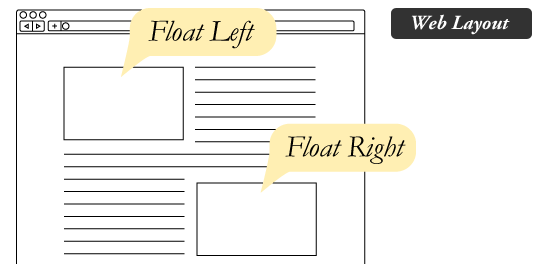
\includegraphics[width=\textwidth]{css-floats}
    \caption{\idx{CSS} floats}
    \label{fig:css-floats}
  \end{figure}
  
  The \idc{clear} property allows to specify not to wrap the element around another floated element; instead it is placed below those elements.
  It supports \idc{left} and \idc{right} values to \emph{clear} all elements floated at that side, or \idc{both} to \emph{clear} any floated elements.
  \item[Absolute positioning] An absolutely positioned element is taken out of the normal flow and effectively ignored by other non-descendant elements, so it has no effect on other items positions.
  Its position is calculated using the \idc{top}, \idc{bottom}, \idc{left} and \idc{right} properties with respect to the first ascendant (closer) that has a \idc{position} value set to other than \idc{static}.
  Since the \idc{relative} value is almost exactly as the \idc{static} value, it is often used to mark the ascendant as the reference.
  
  There is another type of absolute positioning: the \idc{fixed} value works as \idc{absolute}, but it retains its position even when the document is scrolled.
  This is used to achieve a sticky element effect in a page.
\end{description}

Those properties are enough to place an element in the two-dimensional surface that is the document.
However, \ida{CSS} 2.1 introduces another dimension to decide which box must be drawn last when boxes overlap visually.
The order is determined by the position of the boxes in this \emph{z-axis}.

The \idc{z-index} property can be set to any integer (including negatives) to manually set the stack order of that element.
When the page is rendered, elements with greater stack order are drawn in front of other elements with a lower stack order.
However, this \idc{z-index} property is only taken into account when the element is positioned\footnote{A positioned element is any element which its \idc{position} property is set to other than the default \idc{static} value.}.

Usually this property is not needed, but in complex cases it can be handy.
By default, elements are rendered in order of appearance in the \ida{HTML} source file; i.e., if any overlapping occurs, the last element should be drawn on top.
So the \idc{z-index} property is mainly used to revert that behavior.

One side effect of this property is that when an element is positioned, a new \emph{stacking context} is created, completely independent from the its siblings.
This means that the stack order of all child elements now refers to the parent element instead of to the whole document.

Moreover, a child element can only be positioned between its own siblings; respect the parent siblings a child element always have the parent stack order.
For practical purposes, this limits the \idc{z-index} usefulness: if an element is positioned on top of another element, children of the latter can never be positioned on top of the former element.

% subsubsection positioning (end)

\subsubsection{The Box Model} % (fold)
\label{ssub:boxmodel}

\begin{wrapfigure}{r}{0.5\textwidth}
  \centering
    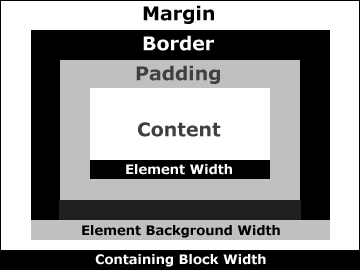
\includegraphics[width=.48\textwidth]{css-boxmodel}
  \caption{\idx{CSS} box model}
  \label{fig:css-boxmodel}
\end{wrapfigure}

In \ida{CSS} each element is treated as a rectangular box.
That box consists of several components, so the final looks and dimensions are defined by the resulting composition of those components.
Figure~\vref{fig:css-boxmodel} and Figure~\vref{fig:css-boxmodel-3d}\footnote{Original image from: \url{http://www.hicksdesign.co.uk/boxmodel/}.} break down a box into its different components.

\begin{figure}[htbp]
  \centering
    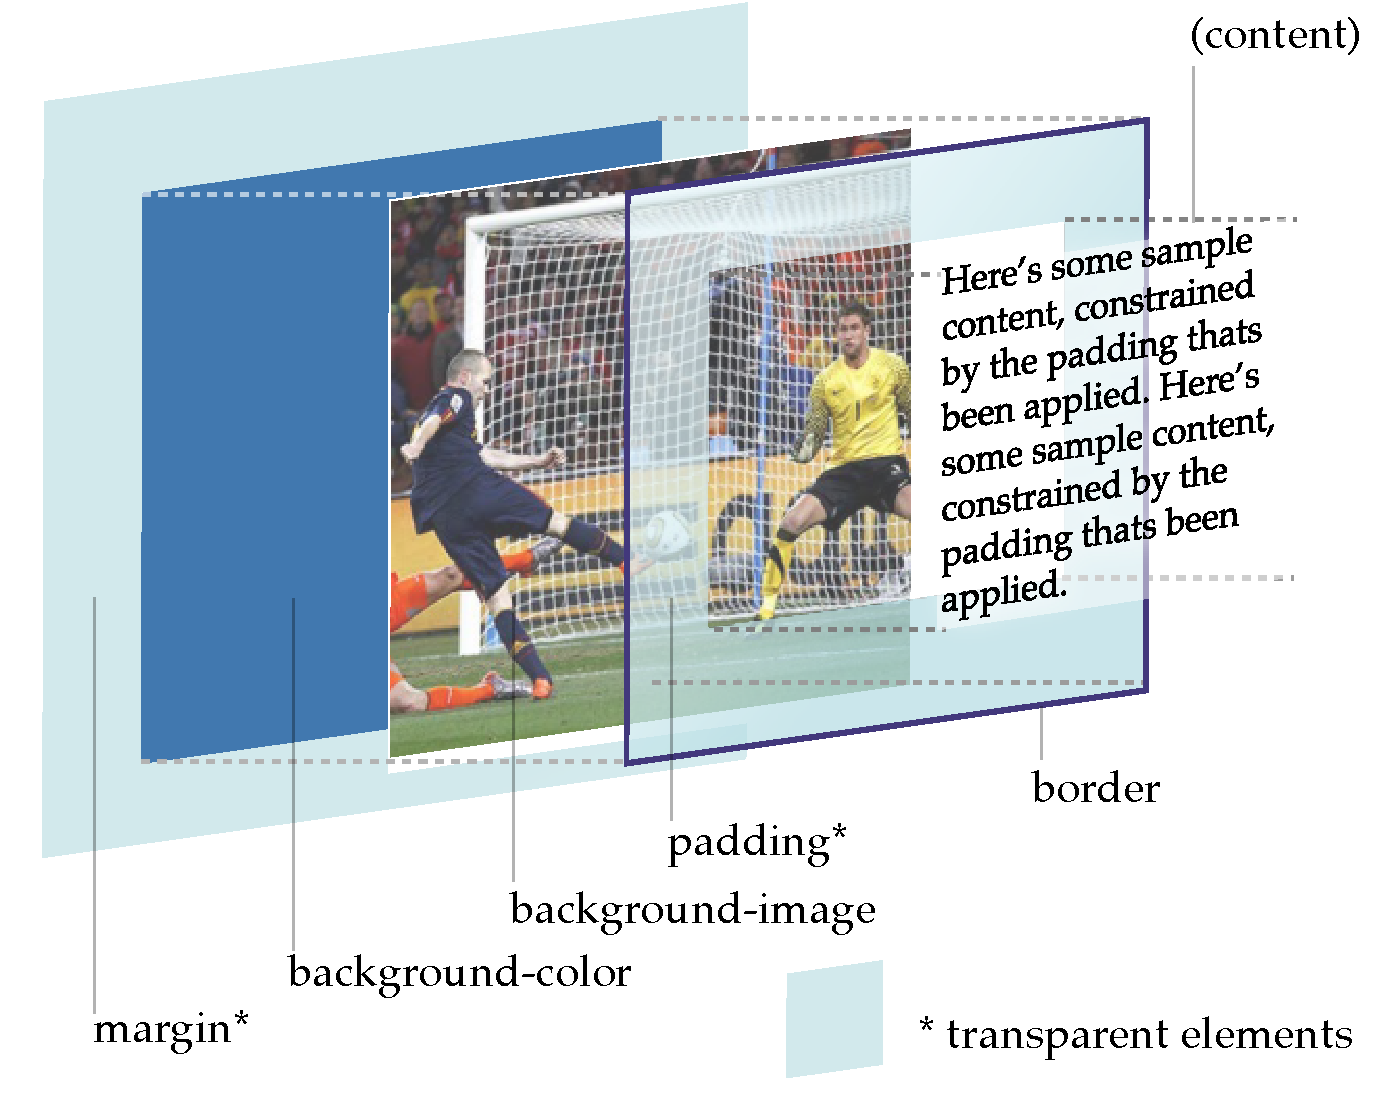
\includegraphics[width=0.9\textwidth]{css-boxmodel-3d}
  \caption{\idx{CSS} box model in 3D}
  \label{fig:css-boxmodel-3d}
\end{figure}

Each component completely encloses the preceded component like a matryoshka doll.
Therefore, its dimensions must be equal or greater than the enclosed component.
These four components can be explained as:

\begin{description}
  \item[Content] is the actual content for that element, including the text and other child elements.
  The \idc{height} and \idc{width} \ida{CSS} properties set these dimensions.
  \item[Padding] is the transparent space surrounding the content, making room between it and the border.
  Different values can be specified for the top, bottom, left and right spaces.
  \item[Border] is the delimiter that marks off the visual boundaries of the box, and it can have several styles and colors.
  As with \idc{padding}, different values can be specified for the top, bottom, left and right borders.
  \item[Margin] is the transparent space surrounding the rest of the elements, and it is usually reserved to provide a visual separation between other elements.
  As with \idc{padding} and \idc{border}, different values can be specified for the top, bottom, left and right spaces.
\end{description}

Any of those elements can have zero dimensions, in that they do not increment the box size.
The \idc{margin} property can even have a negative value, in that case the box is pushed to that direction.
An element's background is painted between the border boundaries, including \emph{behind} the border itself, and excluding the margin space.

Traditionally, working with \ida{CSS} dimensions has been a painful experience because in \ida{IE} the \idc{width} property did not set the content width but the background width.
Newer versions of \ida{IE} (\ida{IE}6+) still exhibit this behavior bug for compatibility reasons, but only if the page triggers the Quirks Mode.
The best solution is to ensure that the browser use the Standards Mode by writing correct \ida{HTML} source code, instead of adding a bunch of empty elements trying to circumvent this issue.

Sometimes the content of an element is bigger than the allocated size for that element.
The \idc{overflow} property defines what to do in those occasions.
By default it has a value of \idc{visible}, allowing the content to be drawn outside the box, but it also accepts \idc{hidden} (clipping it and hiding the overflow content), \idc{scroll} (giving a scroll bar to show the overflow content) and \idc{auto} (like \idc{scroll} but only showing the bar when there is overflow content).

Finally, it is important to note that, although those components work as intended in elements with its \idc{display} property set to \idc{block}, it is quite erratic with inline elements.
The \idc{height} and \idc{width} properties are completely ignored: the height is calculated by the \idc{line-height} property and the width by the content itself.

The \idc{padding} and \idc{margin} properties work, but only affecting the surrounding elements in the horizontal direction, not the vertical direction.
Though, \idc{border} works as intended.
In any case it is clear that inline elements should only be used for text.

% subsubsection boxmodel (end)

\subsubsection{Values and Units} % (fold)
\label{ssub:valuesunits}

Most numeric values are composed by a float number and the identifier for the chosen unit.
Several units are available to specify lengths, some of them are absolute and others are relative.
Absolute units include centimeters (cm), millimeters (mm), inches (in), points (1 pt = 1/72 in) and picas (1 pc = 12 pt).

However relative units are preferred, because they will more easily scale from one medium (device) to another.
The most widely used are px (pixels) and em.
Pixels are relative because the actual size depends on the size of the pixel in the screen device, and it is the most popular way of specifying component sizes.

In turn, em it is defined as the font size of the element, but when it is used in the \idc{font-size} property it refers to the font size of the parent element.
It is therefore preferred for setting font sizes and other typographical properties, like the line height.

The last way of specifying sizes is using percentages (a number plus the `\%' symbol).
However, those percentages are defined upon different properties depending on which property are applied.

Most of the time it refers to the value of the same property on the parent (equals 100\%), e.g., when setting \idc{height}, \idc{width} or \idc{font-size}.
Some properties use another property value as a reference, e.g., spacing properties like \idc{top} or \idc{margin} refers to the \idc{width} and \idc{height} depending on their affecting dimension.
In some typographical properties it refers instead to the current font size, e.g., when setting \idc{line-height}.

Hence, percentages can be used in fluid layouts for almost everything.
Several reasons make it the recommended unit.
Accessibility is the main issue, because the user browser can define different sizes.
But it has other advantages too, such as adapting dynamically to disparate screens or resizing windows.

Colors are usually specified following an hexadecimal \ida{RGB} notation: first the `\#' character, then three hexadecimal numbers between \texttt{00} and \texttt{FF} defining the \emph{amount} of each primary color.
For example, \texttt{\#FFC0CB} represents the pink color, and it is formed by 255 (\texttt{FF}) red, 192 (\texttt{C0}) green and 203 (\texttt{CB}) blue.

Some popular colors can also be specified using a keyword, such as \texttt{white} or \texttt{black}.
Other useful keyword is \texttt{transparent}, that declares that the element property has to be completely transparent.

In \ida{CSS} 3 another notation called \ida{RGBA} is available, with an additional value that declared the \emph{opacity} of that color.
In that notation, though, amounts have to be in decimal notation, e.g. a pink color at 50\% opacity is defined as \texttt{rgba(255,192,203,0.5)}.

% subsubsection valuesunits (end)

% subsection css (end)